\documentclass[twoside]{book}

% Packages required by doxygen
\usepackage{fixltx2e}
\usepackage{calc}
\usepackage{doxygen}
\usepackage[export]{adjustbox} % also loads graphicx
\usepackage{graphicx}
\usepackage[utf8]{inputenc}
\usepackage{makeidx}
\usepackage{multicol}
\usepackage{multirow}
\PassOptionsToPackage{warn}{textcomp}
\usepackage{textcomp}
\usepackage[nointegrals]{wasysym}
\usepackage[table]{xcolor}

% NLS support packages
\usepackage{hfont}

% Font selection
\usepackage[T1]{fontenc}
\usepackage[scaled=.90]{helvet}
\usepackage{courier}
\usepackage{amssymb}
\usepackage{sectsty}
\renewcommand{\familydefault}{\sfdefault}
\allsectionsfont{%
  \fontseries{bc}\selectfont%
  \color{darkgray}%
}
\renewcommand{\DoxyLabelFont}{%
  \fontseries{bc}\selectfont%
  \color{darkgray}%
}
\newcommand{\+}{\discretionary{\mbox{\scriptsize$\hookleftarrow$}}{}{}}

% Page & text layout
\usepackage{geometry}
\geometry{%
  a4paper,%
  top=2.5cm,%
  bottom=2.5cm,%
  left=2.5cm,%
  right=2.5cm%
}
\tolerance=750
\hfuzz=15pt
\hbadness=750
\setlength{\emergencystretch}{15pt}
\setlength{\parindent}{0cm}
\setlength{\parskip}{3ex plus 2ex minus 2ex}
\makeatletter
\renewcommand{\paragraph}{%
  \@startsection{paragraph}{4}{0ex}{-1.0ex}{1.0ex}{%
    \normalfont\normalsize\bfseries\SS@parafont%
  }%
}
\renewcommand{\subparagraph}{%
  \@startsection{subparagraph}{5}{0ex}{-1.0ex}{1.0ex}{%
    \normalfont\normalsize\bfseries\SS@subparafont%
  }%
}
\makeatother

% Headers & footers
\usepackage{fancyhdr}
\pagestyle{fancyplain}
\fancyhead[LE]{\fancyplain{}{\bfseries\thepage}}
\fancyhead[CE]{\fancyplain{}{}}
\fancyhead[RE]{\fancyplain{}{\bfseries\leftmark}}
\fancyhead[LO]{\fancyplain{}{\bfseries\rightmark}}
\fancyhead[CO]{\fancyplain{}{}}
\fancyhead[RO]{\fancyplain{}{\bfseries\thepage}}
\fancyfoot[LE]{\fancyplain{}{}}
\fancyfoot[CE]{\fancyplain{}{}}
\fancyfoot[RE]{\fancyplain{}{\bfseries\scriptsize 다음에 의해 생성됨 \+:  Doxygen }}
\fancyfoot[LO]{\fancyplain{}{\bfseries\scriptsize 다음에 의해 생성됨 \+:  Doxygen }}
\fancyfoot[CO]{\fancyplain{}{}}
\fancyfoot[RO]{\fancyplain{}{}}
\renewcommand{\footrulewidth}{0.4pt}
\renewcommand{\chaptermark}[1]{%
  \markboth{#1}{}%
}
\renewcommand{\sectionmark}[1]{%
  \markright{\thesection\ #1}%
}

% Indices & bibliography
\usepackage{natbib}
\usepackage[titles]{tocloft}
\setcounter{tocdepth}{3}
\setcounter{secnumdepth}{5}
\makeindex

% Hyperlinks (required, but should be loaded last)
\usepackage{ifpdf}
\ifpdf
  \usepackage[pdftex,pagebackref=true]{hyperref}
\else
  \usepackage[ps2pdf,pagebackref=true]{hyperref}
\fi
\hypersetup{%
  colorlinks=true,%
  linkcolor=blue,%
  citecolor=blue,%
  unicode%
}

% Custom commands
\newcommand{\clearemptydoublepage}{%
  \newpage{\pagestyle{empty}\cleardoublepage}%
}

\usepackage{caption}
\captionsetup{labelsep=space,justification=centering,font={bf},singlelinecheck=off,skip=4pt,position=top}

%===== C O N T E N T S =====

\begin{document}

% Titlepage & ToC
\hypersetup{pageanchor=false,
             bookmarksnumbered=true,
             pdfencoding=unicode
            }
\pagenumbering{roman}
\begin{titlepage}
\vspace*{7cm}
\begin{center}%
{\Large Mine\+Sweeper }\\
\vspace*{1cm}
{\large 다음에 의해 생성됨 \+:  Doxygen 1.8.11}\\
\end{center}
\end{titlepage}
\clearemptydoublepage
\tableofcontents
\clearemptydoublepage
\pagenumbering{arabic}
\hypersetup{pageanchor=true}

%--- Begin generated contents ---
\chapter{네임스페이스 색인}
\section{패키지}
다음은 패키지들입니다. (가능한한 간략한 설명만을 보여줍니다) \+:\begin{DoxyCompactList}
\item\contentsline{section}{\hyperlink{namespacehufs}{hufs} }{\pageref{namespacehufs}}{}
\item\contentsline{section}{\hyperlink{namespacehufs_1_1cse}{hufs.\+cse} }{\pageref{namespacehufs_1_1cse}}{}
\item\contentsline{section}{\hyperlink{namespacehufs_1_1cse_1_1khk}{hufs.\+cse.\+khk} }{\pageref{namespacehufs_1_1cse_1_1khk}}{}
\end{DoxyCompactList}

\chapter{계통도 색인}
\section{클래스 계통도}
이 상속 목록은 완전하진 않지만 알파벳순으로 대략적으로 정렬되어있습니다.\+:\begin{DoxyCompactList}
\item Action\+Listener\begin{DoxyCompactList}
\item \contentsline{section}{hufs.\+cse.\+khk.\+Minesweeper\+UI}{\pageref{classhufs_1_1cse_1_1khk_1_1_minesweeper_u_i}}{}
\end{DoxyCompactList}
\item Container\+Listener\begin{DoxyCompactList}
\item \contentsline{section}{hufs.\+cse.\+khk.\+Minesweeper\+UI}{\pageref{classhufs_1_1cse_1_1khk_1_1_minesweeper_u_i}}{}
\end{DoxyCompactList}
\item \contentsline{section}{hufs.\+cse.\+khk.\+main}{\pageref{classhufs_1_1cse_1_1khk_1_1main}}{}
\item \contentsline{section}{hufs.\+cse.\+khk.\+Minesweeper}{\pageref{classhufs_1_1cse_1_1khk_1_1_minesweeper}}{}
\item \contentsline{section}{hufs.\+cse.\+khk.\+Rank}{\pageref{classhufs_1_1cse_1_1khk_1_1_rank}}{}
\item Runnable\begin{DoxyCompactList}
\item \contentsline{section}{hufs.\+cse.\+khk.\+Timer}{\pageref{classhufs_1_1cse_1_1khk_1_1_timer}}{}
\end{DoxyCompactList}
\item J\+Frame\begin{DoxyCompactList}
\item \contentsline{section}{hufs.\+cse.\+khk.\+Minesweeper\+UI}{\pageref{classhufs_1_1cse_1_1khk_1_1_minesweeper_u_i}}{}
\item \contentsline{section}{hufs.\+cse.\+khk.\+Timer}{\pageref{classhufs_1_1cse_1_1khk_1_1_timer}}{}
\end{DoxyCompactList}
\end{DoxyCompactList}

\chapter{클래스 색인}
\section{클래스 목록}
다음은 클래스, 구조체, 공용체 그리고 인터페이스들입니다. (간략한 설명만을 보여줍니다) \+:\begin{DoxyCompactList}
\item\contentsline{section}{\hyperlink{classhufs_1_1cse_1_1khk_1_1main}{hufs.\+cse.\+khk.\+main} \\*Run Class }{\pageref{classhufs_1_1cse_1_1khk_1_1main}}{}
\item\contentsline{section}{\hyperlink{classhufs_1_1cse_1_1khk_1_1_minesweeper}{hufs.\+cse.\+khk.\+Minesweeper} \\*\hyperlink{classhufs_1_1cse_1_1khk_1_1_minesweeper}{Minesweeper} \+: \hyperlink{classhufs_1_1cse_1_1khk_1_1_minesweeper}{Minesweeper} data class }{\pageref{classhufs_1_1cse_1_1khk_1_1_minesweeper}}{}
\item\contentsline{section}{\hyperlink{classhufs_1_1cse_1_1khk_1_1_minesweeper_u_i}{hufs.\+cse.\+khk.\+Minesweeper\+UI} \\*\hyperlink{classhufs_1_1cse_1_1khk_1_1_minesweeper}{Minesweeper} UI }{\pageref{classhufs_1_1cse_1_1khk_1_1_minesweeper_u_i}}{}
\item\contentsline{section}{\hyperlink{classhufs_1_1cse_1_1khk_1_1_rank}{hufs.\+cse.\+khk.\+Rank} \\*\hyperlink{classhufs_1_1cse_1_1khk_1_1_rank}{Rank} \+: User Ranking Class }{\pageref{classhufs_1_1cse_1_1khk_1_1_rank}}{}
\item\contentsline{section}{\hyperlink{classhufs_1_1cse_1_1khk_1_1_timer}{hufs.\+cse.\+khk.\+Timer} \\*\hyperlink{classhufs_1_1cse_1_1khk_1_1_timer}{Timer} Class }{\pageref{classhufs_1_1cse_1_1khk_1_1_timer}}{}
\end{DoxyCompactList}

\chapter{파일 색인}
\section{파일 목록}
다음은 모든 파일에 대한 목록입니다. (간략한 설명만을 보여줍니다) \+:\begin{DoxyCompactList}
\item\contentsline{section}{C\+:/pub/\+Workspace\+\_\+\+S\+E/\+Report3\+\_\+test3/src/hufs/cse/khk/\hyperlink{main_8java}{main.\+java} }{\pageref{main_8java}}{}
\item\contentsline{section}{C\+:/pub/\+Workspace\+\_\+\+S\+E/\+Report3\+\_\+test3/src/hufs/cse/khk/\hyperlink{_minesweeper_8java}{Minesweeper.\+java} }{\pageref{_minesweeper_8java}}{}
\item\contentsline{section}{C\+:/pub/\+Workspace\+\_\+\+S\+E/\+Report3\+\_\+test3/src/hufs/cse/khk/\hyperlink{_minesweeper_u_i_8java}{Minesweeper\+U\+I.\+java} }{\pageref{_minesweeper_u_i_8java}}{}
\item\contentsline{section}{C\+:/pub/\+Workspace\+\_\+\+S\+E/\+Report3\+\_\+test3/src/hufs/cse/khk/\hyperlink{_rank_8java}{Rank.\+java} }{\pageref{_rank_8java}}{}
\item\contentsline{section}{C\+:/pub/\+Workspace\+\_\+\+S\+E/\+Report3\+\_\+test3/src/hufs/cse/khk/\hyperlink{_timer_8java}{Timer.\+java} }{\pageref{_timer_8java}}{}
\end{DoxyCompactList}

\chapter{네임스페이스 문서화}
\hypertarget{namespacehufs}{}\section{hufs 패키지}
\label{namespacehufs}\index{hufs@{hufs}}
\subsection*{패키지}
\begin{DoxyCompactItemize}
\item 
package \hyperlink{namespacehufs_1_1cse}{cse}
\end{DoxyCompactItemize}

\hypertarget{namespacehufs_1_1cse}{}\section{hufs.\+cse 패키지}
\label{namespacehufs_1_1cse}\index{hufs.\+cse@{hufs.\+cse}}
\subsection*{패키지}
\begin{DoxyCompactItemize}
\item 
package \hyperlink{namespacehufs_1_1cse_1_1khk}{khk}
\end{DoxyCompactItemize}

\hypertarget{namespacehufs_1_1cse_1_1khk}{}\section{hufs.\+cse.\+khk 패키지}
\label{namespacehufs_1_1cse_1_1khk}\index{hufs.\+cse.\+khk@{hufs.\+cse.\+khk}}
\subsection*{클래스}
\begin{DoxyCompactItemize}
\item 
class \hyperlink{classhufs_1_1cse_1_1khk_1_1main}{main}
\begin{DoxyCompactList}\small\item\em Run Class. \end{DoxyCompactList}\item 
class \hyperlink{classhufs_1_1cse_1_1khk_1_1_minesweeper}{Minesweeper}
\begin{DoxyCompactList}\small\item\em \hyperlink{classhufs_1_1cse_1_1khk_1_1_minesweeper}{Minesweeper} \+: \hyperlink{classhufs_1_1cse_1_1khk_1_1_minesweeper}{Minesweeper} data class. \end{DoxyCompactList}\item 
class \hyperlink{classhufs_1_1cse_1_1khk_1_1_minesweeper_u_i}{Minesweeper\+UI}
\begin{DoxyCompactList}\small\item\em \hyperlink{classhufs_1_1cse_1_1khk_1_1_minesweeper}{Minesweeper} UI. \end{DoxyCompactList}\item 
class \hyperlink{classhufs_1_1cse_1_1khk_1_1_rank}{Rank}
\begin{DoxyCompactList}\small\item\em \hyperlink{classhufs_1_1cse_1_1khk_1_1_rank}{Rank} \+: User Ranking Class. \end{DoxyCompactList}\item 
class \hyperlink{classhufs_1_1cse_1_1khk_1_1_timer}{Timer}
\begin{DoxyCompactList}\small\item\em \hyperlink{classhufs_1_1cse_1_1khk_1_1_timer}{Timer} Class. \end{DoxyCompactList}\end{DoxyCompactItemize}

\chapter{클래스 문서화}
\hypertarget{classhufs_1_1cse_1_1khk_1_1main}{}\section{hufs.\+cse.\+khk.\+main 클래스 참조}
\label{classhufs_1_1cse_1_1khk_1_1main}\index{hufs.\+cse.\+khk.\+main@{hufs.\+cse.\+khk.\+main}}


Run Class.  


\subsection*{정적 Public 멤버 함수}
\begin{DoxyCompactItemize}
\item 
static void \hyperlink{classhufs_1_1cse_1_1khk_1_1main_a89796462e353c08e63fc0acf72500937}{main} (String\mbox{[}$\,$\mbox{]} args)
\end{DoxyCompactItemize}


\subsection{상세한 설명}
Run Class. 

\begin{DoxyAuthor}{작성자}
gudrbscse 
\end{DoxyAuthor}


main.\+java 파일의 9 번째 라인에서 정의되었습니다.



\subsection{생성자 \& 소멸자 문서화}
\index{hufs\+::cse\+::khk\+::main@{hufs\+::cse\+::khk\+::main}!main@{main}}
\index{main@{main}!hufs\+::cse\+::khk\+::main@{hufs\+::cse\+::khk\+::main}}
\subsubsection[{\texorpdfstring{main(\+String[] args)}{main(String[] args)}}]{\setlength{\rightskip}{0pt plus 5cm}static void hufs.\+cse.\+khk.\+main.\+main (
\begin{DoxyParamCaption}
\item[{String\mbox{[}$\,$\mbox{]}}]{args}
\end{DoxyParamCaption}
)\hspace{0.3cm}{\ttfamily [static]}}\hypertarget{classhufs_1_1cse_1_1khk_1_1main_a89796462e353c08e63fc0acf72500937}{}\label{classhufs_1_1cse_1_1khk_1_1main_a89796462e353c08e63fc0acf72500937}


main.\+java 파일의 10 번째 라인에서 정의되었습니다.


\begin{DoxyCode}
10                                            \{
11         Minesweeper m = \textcolor{keyword}{new} Minesweeper();
12     \}
\end{DoxyCode}


이 클래스에 대한 문서화 페이지는 다음의 파일로부터 생성되었습니다.\+:\begin{DoxyCompactItemize}
\item 
C\+:/pub/\+Workspace\+\_\+\+S\+E/\+Report3\+\_\+test3/src/hufs/cse/khk/\hyperlink{main_8java}{main.\+java}\end{DoxyCompactItemize}

\hypertarget{classhufs_1_1cse_1_1khk_1_1_minesweeper}{}\section{hufs.\+cse.\+khk.\+Minesweeper 클래스 참조}
\label{classhufs_1_1cse_1_1khk_1_1_minesweeper}\index{hufs.\+cse.\+khk.\+Minesweeper@{hufs.\+cse.\+khk.\+Minesweeper}}


\hyperlink{classhufs_1_1cse_1_1khk_1_1_minesweeper}{Minesweeper} \+: \hyperlink{classhufs_1_1cse_1_1khk_1_1_minesweeper}{Minesweeper} data class.  


\subsection*{Public 멤버 함수}
\begin{DoxyCompactItemize}
\item 
\hyperlink{classhufs_1_1cse_1_1khk_1_1_minesweeper_ae984f5f16cc438084f11ffe5fa9cf4e8}{Minesweeper} ()
\begin{DoxyCompactList}\small\item\em Create UI. \end{DoxyCompactList}\end{DoxyCompactItemize}


\subsection{상세한 설명}
\hyperlink{classhufs_1_1cse_1_1khk_1_1_minesweeper}{Minesweeper} \+: \hyperlink{classhufs_1_1cse_1_1khk_1_1_minesweeper}{Minesweeper} data class. 

\begin{DoxyAuthor}{작성자}
gudrbscse
\end{DoxyAuthor}
\hyperlink{classhufs_1_1cse_1_1khk_1_1_minesweeper}{Minesweeper} 클래스 프로그램의 데이터 클래스로, UI 클래스 및 \hyperlink{classhufs_1_1cse_1_1khk_1_1_minesweeper}{Minesweeper} Game 에 필요한 데이터가 들어간다. 

Minesweeper.\+java 파일의 21 번째 라인에서 정의되었습니다.



\subsection{생성자 \& 소멸자 문서화}
\index{hufs\+::cse\+::khk\+::\+Minesweeper@{hufs\+::cse\+::khk\+::\+Minesweeper}!Minesweeper@{Minesweeper}}
\index{Minesweeper@{Minesweeper}!hufs\+::cse\+::khk\+::\+Minesweeper@{hufs\+::cse\+::khk\+::\+Minesweeper}}
\subsubsection[{\texorpdfstring{Minesweeper()}{Minesweeper()}}]{\setlength{\rightskip}{0pt plus 5cm}hufs.\+cse.\+khk.\+Minesweeper.\+Minesweeper (
\begin{DoxyParamCaption}
{}
\end{DoxyParamCaption}
)}\hypertarget{classhufs_1_1cse_1_1khk_1_1_minesweeper_ae984f5f16cc438084f11ffe5fa9cf4e8}{}\label{classhufs_1_1cse_1_1khk_1_1_minesweeper_ae984f5f16cc438084f11ffe5fa9cf4e8}


Create UI. 

Minsweeper\+UI 클래스를 생성하여 지뢰찾기 G\+UI 게임을 실행한다. 

Minesweeper.\+java 파일의 44 번째 라인에서 정의되었습니다.


\begin{DoxyCode}
44                         \{
45         minesweeperui = \textcolor{keyword}{new} MinesweeperUI(\textcolor{keyword}{this});
46     \}       
\end{DoxyCode}


이 클래스에 대한 문서화 페이지는 다음의 파일로부터 생성되었습니다.\+:\begin{DoxyCompactItemize}
\item 
C\+:/pub/\+Workspace\+\_\+\+S\+E/\+Report3\+\_\+test3/src/hufs/cse/khk/\hyperlink{_minesweeper_8java}{Minesweeper.\+java}\end{DoxyCompactItemize}

\hypertarget{classhufs_1_1cse_1_1khk_1_1_minesweeper_u_i}{}\section{hufs.\+cse.\+khk.\+Minesweeper\+UI 클래스 참조}
\label{classhufs_1_1cse_1_1khk_1_1_minesweeper_u_i}\index{hufs.\+cse.\+khk.\+Minesweeper\+UI@{hufs.\+cse.\+khk.\+Minesweeper\+UI}}


\hyperlink{classhufs_1_1cse_1_1khk_1_1_minesweeper}{Minesweeper} UI.  


hufs.\+cse.\+khk.\+Minesweeper\+U\+I에 대한 상속 다이어그램 \+: \begin{figure}[H]
\begin{center}
\leavevmode
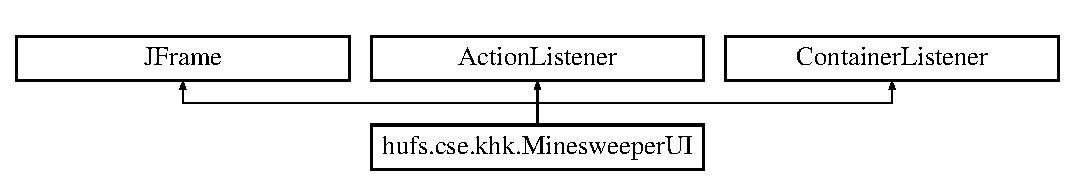
\includegraphics[height=2.000000cm]{classhufs_1_1cse_1_1khk_1_1_minesweeper_u_i}
\end{center}
\end{figure}
\subsection*{클래스}
\begin{DoxyCompactItemize}
\item 
class {\bfseries Customization}
\begin{DoxyCompactList}\small\item\em Customize Mode. \end{DoxyCompactList}\item 
class {\bfseries Mouse\+Handler}
\begin{DoxyCompactList}\small\item\em Mouse Handler. \end{DoxyCompactList}\end{DoxyCompactItemize}
\subsection*{Public 멤버 함수}
\begin{DoxyCompactItemize}
\item 
\hyperlink{classhufs_1_1cse_1_1khk_1_1_minesweeper_u_i_aac09dd5162a5dc77642c78c0cc5352f4}{Minesweeper\+UI} (\hyperlink{classhufs_1_1cse_1_1khk_1_1_minesweeper}{Minesweeper} minesweeper)
\begin{DoxyCompactList}\small\item\em 생성자 \end{DoxyCompactList}\item 
void \hyperlink{classhufs_1_1cse_1_1khk_1_1_minesweeper_u_i_a9d9ff2e282de36230ad02df0c9b53809}{setmenu} ()
\begin{DoxyCompactList}\small\item\em set menu \end{DoxyCompactList}\item 
void \hyperlink{classhufs_1_1cse_1_1khk_1_1_minesweeper_u_i_a9a871b3969d0f0c00cf420902d09cc18}{setpanel} (int level, int setr, int setc, int setm)
\begin{DoxyCompactList}\small\item\em Set Panel. \end{DoxyCompactList}\item 
void \hyperlink{classhufs_1_1cse_1_1khk_1_1_minesweeper_u_i_acf0fc1f12fcce4b62901961c425febb7}{set\+Image\+Icon} ()
\begin{DoxyCompactList}\small\item\em Set Image\+Icon. \end{DoxyCompactList}\item 
void \hyperlink{classhufs_1_1cse_1_1khk_1_1_minesweeper_u_i_a137388c25def2c90fe13e34d6234207d}{reset} ()
\begin{DoxyCompactList}\small\item\em Reset. \end{DoxyCompactList}\item 
void \hyperlink{classhufs_1_1cse_1_1khk_1_1_minesweeper_u_i_a1a12092d57cfb53d87a5c96672a984d9}{component\+Added} (Container\+Event ce)
\item 
void \hyperlink{classhufs_1_1cse_1_1khk_1_1_minesweeper_u_i_a1270d3daaaf848642adc88f5f735eb9f}{component\+Removed} (Container\+Event ce)
\item 
void \hyperlink{classhufs_1_1cse_1_1khk_1_1_minesweeper_u_i_a896a8e57a116a0b4b43fb88b575ab5b8}{action\+Performed} (Action\+Event ae)
\item 
void \hyperlink{classhufs_1_1cse_1_1khk_1_1_minesweeper_u_i_a4bb7cb917ff08bb92313768edfb9e976}{win\+\_\+check} ()
\begin{DoxyCompactList}\small\item\em win check \end{DoxyCompactList}\item 
void \hyperlink{classhufs_1_1cse_1_1khk_1_1_minesweeper_u_i_a11c77f8dd3a89c96b8a32c64f4e2aef5}{Search\+Mine} (Mouse\+Event e)
\begin{DoxyCompactList}\small\item\em Search Mine. \end{DoxyCompactList}\item 
void \hyperlink{classhufs_1_1cse_1_1khk_1_1_minesweeper_u_i_ac9d8adecf10f5e6f203fc979fe032963}{dfs} (int row, int col)
\begin{DoxyCompactList}\small\item\em dfs func \end{DoxyCompactList}\item 
void \hyperlink{classhufs_1_1cse_1_1khk_1_1_minesweeper_u_i_a87c73fb5d1f5cc33c8ca0a7b337849d3}{calculation} ()
\begin{DoxyCompactList}\small\item\em calculate value \end{DoxyCompactList}\item 
void \hyperlink{classhufs_1_1cse_1_1khk_1_1_minesweeper_u_i_a9649859be1093b220e48f02b27171a9d}{setmine} ()
\begin{DoxyCompactList}\small\item\em Set Mine. \end{DoxyCompactList}\end{DoxyCompactItemize}


\subsection{상세한 설명}
\hyperlink{classhufs_1_1cse_1_1khk_1_1_minesweeper}{Minesweeper} UI. 

\begin{DoxyAuthor}{작성자}
gudrbscse
\end{DoxyAuthor}
지뢰찾기의 G\+UI Class 이다. 

Minesweeper\+U\+I.\+java 파일의 19 번째 라인에서 정의되었습니다.



\subsection{생성자 \& 소멸자 문서화}
\index{hufs\+::cse\+::khk\+::\+Minesweeper\+UI@{hufs\+::cse\+::khk\+::\+Minesweeper\+UI}!Minesweeper\+UI@{Minesweeper\+UI}}
\index{Minesweeper\+UI@{Minesweeper\+UI}!hufs\+::cse\+::khk\+::\+Minesweeper\+UI@{hufs\+::cse\+::khk\+::\+Minesweeper\+UI}}
\subsubsection[{\texorpdfstring{Minesweeper\+U\+I(\+Minesweeper minesweeper)}{MinesweeperUI(Minesweeper minesweeper)}}]{\setlength{\rightskip}{0pt plus 5cm}hufs.\+cse.\+khk.\+Minesweeper\+U\+I.\+Minesweeper\+UI (
\begin{DoxyParamCaption}
\item[{{\bf Minesweeper}}]{minesweeper}
\end{DoxyParamCaption}
)}\hypertarget{classhufs_1_1cse_1_1khk_1_1_minesweeper_u_i_aac09dd5162a5dc77642c78c0cc5352f4}{}\label{classhufs_1_1cse_1_1khk_1_1_minesweeper_u_i_aac09dd5162a5dc77642c78c0cc5352f4}


생성자 


\begin{DoxyParams}{매개변수}
{\em minesweeper} & \\
\hline
\end{DoxyParams}
minesweeper 클래스를 통해서 data 변수들을 받는다. 

Minesweeper\+U\+I.\+java 파일의 40 번째 라인에서 정의되었습니다.



다음을 참조함 \+:  hufs.\+cse.\+khk.\+Minesweeper\+U\+I.\+action\+Performed(), hufs.\+cse.\+khk.\+Minesweeper\+U\+I.\+reset(), hufs.\+cse.\+khk.\+Minesweeper\+U\+I.\+set\+Image\+Icon(), hufs.\+cse.\+khk.\+Minesweeper\+U\+I.\+setmenu(), hufs.\+cse.\+khk.\+Minesweeper\+U\+I.\+setpanel(), hufs.\+cse.\+khk.\+Timer.\+stop().


\begin{DoxyCode}
40                                                   \{
41         super(\textcolor{stringliteral}{"지뢰찾기"});
42         this.minesweeper = minesweeper;
43         
44         setLocation(900, 300);
45         \hyperlink{classhufs_1_1cse_1_1khk_1_1_minesweeper_u_i_acf0fc1f12fcce4b62901961c425febb7}{setImageIcon}();
46         \hyperlink{classhufs_1_1cse_1_1khk_1_1_minesweeper_u_i_a9a871b3969d0f0c00cf420902d09cc18}{setpanel}(1, 0, 0, 0);
47         \hyperlink{classhufs_1_1cse_1_1khk_1_1_minesweeper_u_i_a9d9ff2e282de36230ad02df0c9b53809}{setmenu}();
48         minesweeper.timer = \textcolor{keyword}{new} Timer(\textcolor{keyword}{this});
49  
50         \hyperlink{classhufs_1_1cse_1_1khk_1_1_minesweeper_u_i_a137388c25def2c90fe13e34d6234207d}{reset}.addActionListener(\textcolor{keyword}{new} ActionListener() \{
51             \textcolor{keyword}{public} \textcolor{keywordtype}{void} \hyperlink{classhufs_1_1cse_1_1khk_1_1_minesweeper_u_i_a896a8e57a116a0b4b43fb88b575ab5b8}{actionPerformed}(ActionEvent ae) \{
52                 \textcolor{keywordflow}{try} \{
53                     minesweeper.timer.\hyperlink{classhufs_1_1cse_1_1khk_1_1_timer_a5ab9e7bd1e1b1f74604887cd99b27972}{stop}();
54                     \hyperlink{classhufs_1_1cse_1_1khk_1_1_minesweeper_u_i_a9a871b3969d0f0c00cf420902d09cc18}{setpanel}(minesweeper.minelevel, minesweeper.savedblockr, minesweeper.
      savedblockc, minesweeper.savednum\_of\_mine);
55                 \} \textcolor{keywordflow}{catch} (Exception ex) \{
56                     \hyperlink{classhufs_1_1cse_1_1khk_1_1_minesweeper_u_i_a9a871b3969d0f0c00cf420902d09cc18}{setpanel}(minesweeper.minelevel, minesweeper.savedblockr, minesweeper.
      savedblockc, minesweeper.savednum\_of\_mine);
57                 \}
58                 \hyperlink{classhufs_1_1cse_1_1khk_1_1_minesweeper_u_i_a137388c25def2c90fe13e34d6234207d}{reset}();
59             \}
60         \});
61         setDefaultCloseOperation(EXIT\_ON\_CLOSE);
62     \}
\end{DoxyCode}


\subsection{멤버 함수 문서화}
\index{hufs\+::cse\+::khk\+::\+Minesweeper\+UI@{hufs\+::cse\+::khk\+::\+Minesweeper\+UI}!action\+Performed@{action\+Performed}}
\index{action\+Performed@{action\+Performed}!hufs\+::cse\+::khk\+::\+Minesweeper\+UI@{hufs\+::cse\+::khk\+::\+Minesweeper\+UI}}
\subsubsection[{\texorpdfstring{action\+Performed(\+Action\+Event ae)}{actionPerformed(ActionEvent ae)}}]{\setlength{\rightskip}{0pt plus 5cm}void hufs.\+cse.\+khk.\+Minesweeper\+U\+I.\+action\+Performed (
\begin{DoxyParamCaption}
\item[{Action\+Event}]{ae}
\end{DoxyParamCaption}
)}\hypertarget{classhufs_1_1cse_1_1khk_1_1_minesweeper_u_i_a896a8e57a116a0b4b43fb88b575ab5b8}{}\label{classhufs_1_1cse_1_1khk_1_1_minesweeper_u_i_a896a8e57a116a0b4b43fb88b575ab5b8}


Minesweeper\+U\+I.\+java 파일의 390 번째 라인에서 정의되었습니다.



다음을 참조함 \+:  hufs.\+cse.\+khk.\+Minesweeper\+U\+I.\+calculation(), hufs.\+cse.\+khk.\+Minesweeper\+U\+I.\+Search\+Mine(), hufs.\+cse.\+khk.\+Minesweeper\+U\+I.\+setmine(), hufs.\+cse.\+khk.\+Timer.\+Start(), hufs.\+cse.\+khk.\+Minesweeper\+U\+I.\+win\+\_\+check().



다음에 의해서 참조됨 \+:  hufs.\+cse.\+khk.\+Minesweeper\+U\+I.\+Minesweeper\+U\+I(), hufs.\+cse.\+khk.\+Minesweeper\+U\+I.\+setmenu(), hufs.\+cse.\+khk.\+Minesweeper\+U\+I.\+setmine().


\begin{DoxyCode}
390                                                 \{
391     \}
\end{DoxyCode}
\index{hufs\+::cse\+::khk\+::\+Minesweeper\+UI@{hufs\+::cse\+::khk\+::\+Minesweeper\+UI}!calculation@{calculation}}
\index{calculation@{calculation}!hufs\+::cse\+::khk\+::\+Minesweeper\+UI@{hufs\+::cse\+::khk\+::\+Minesweeper\+UI}}
\subsubsection[{\texorpdfstring{calculation()}{calculation()}}]{\setlength{\rightskip}{0pt plus 5cm}void hufs.\+cse.\+khk.\+Minesweeper\+U\+I.\+calculation (
\begin{DoxyParamCaption}
{}
\end{DoxyParamCaption}
)}\hypertarget{classhufs_1_1cse_1_1khk_1_1_minesweeper_u_i_a87c73fb5d1f5cc33c8ca0a7b337849d3}{}\label{classhufs_1_1cse_1_1khk_1_1_minesweeper_u_i_a87c73fb5d1f5cc33c8ca0a7b337849d3}


calculate value 

구역 주변에 지뢰가 몇개 있는지 계산하는 함수이다. 0$\sim$8의 값을 가진다. 

Minesweeper\+U\+I.\+java 파일의 560 번째 라인에서 정의되었습니다.



다음에 의해서 참조됨 \+:  hufs.\+cse.\+khk.\+Minesweeper\+U\+I.\+action\+Performed().


\begin{DoxyCode}
560                               \{
561         \textcolor{keywordtype}{int} row, column;
562         \textcolor{keywordflow}{for} (\textcolor{keywordtype}{int} i = 0; i < minesweeper.blockr; i++) \{
563             \textcolor{keywordflow}{for} (\textcolor{keywordtype}{int} j = 0; j < minesweeper.blockc; j++) \{
564                 \textcolor{keywordtype}{int} value = 0;
565                 \textcolor{keywordtype}{int} R, C;
566                 row = i;
567                 column = j;
568                 \textcolor{keywordflow}{if} (minesweeper.countmine[row][column] != -1) \{
569                     \textcolor{keywordflow}{for} (\textcolor{keywordtype}{int} k = 0; k < 8; k++) \{
570                         R = row + minesweeper.r[k];
571                         C = column + minesweeper.c[k];
572  
573                         \textcolor{keywordflow}{if} (R >= 0 && C >= 0 && R < minesweeper.blockr && C < minesweeper.blockc) \{
574                             \textcolor{keywordflow}{if} (minesweeper.countmine[R][C] == -1) \{
575                                 value++;
576                             \}
577                         \}
578                     \}
579                     minesweeper.countmine[row][column] = value;
580                 \}
581             \}
582         \}
583     \}
\end{DoxyCode}
\index{hufs\+::cse\+::khk\+::\+Minesweeper\+UI@{hufs\+::cse\+::khk\+::\+Minesweeper\+UI}!component\+Added@{component\+Added}}
\index{component\+Added@{component\+Added}!hufs\+::cse\+::khk\+::\+Minesweeper\+UI@{hufs\+::cse\+::khk\+::\+Minesweeper\+UI}}
\subsubsection[{\texorpdfstring{component\+Added(\+Container\+Event ce)}{componentAdded(ContainerEvent ce)}}]{\setlength{\rightskip}{0pt plus 5cm}void hufs.\+cse.\+khk.\+Minesweeper\+U\+I.\+component\+Added (
\begin{DoxyParamCaption}
\item[{Container\+Event}]{ce}
\end{DoxyParamCaption}
)}\hypertarget{classhufs_1_1cse_1_1khk_1_1_minesweeper_u_i_a1a12092d57cfb53d87a5c96672a984d9}{}\label{classhufs_1_1cse_1_1khk_1_1_minesweeper_u_i_a1a12092d57cfb53d87a5c96672a984d9}


Minesweeper\+U\+I.\+java 파일의 384 번째 라인에서 정의되었습니다.


\begin{DoxyCode}
384                                                   \{
385     \}
\end{DoxyCode}
\index{hufs\+::cse\+::khk\+::\+Minesweeper\+UI@{hufs\+::cse\+::khk\+::\+Minesweeper\+UI}!component\+Removed@{component\+Removed}}
\index{component\+Removed@{component\+Removed}!hufs\+::cse\+::khk\+::\+Minesweeper\+UI@{hufs\+::cse\+::khk\+::\+Minesweeper\+UI}}
\subsubsection[{\texorpdfstring{component\+Removed(\+Container\+Event ce)}{componentRemoved(ContainerEvent ce)}}]{\setlength{\rightskip}{0pt plus 5cm}void hufs.\+cse.\+khk.\+Minesweeper\+U\+I.\+component\+Removed (
\begin{DoxyParamCaption}
\item[{Container\+Event}]{ce}
\end{DoxyParamCaption}
)}\hypertarget{classhufs_1_1cse_1_1khk_1_1_minesweeper_u_i_a1270d3daaaf848642adc88f5f735eb9f}{}\label{classhufs_1_1cse_1_1khk_1_1_minesweeper_u_i_a1270d3daaaf848642adc88f5f735eb9f}


Minesweeper\+U\+I.\+java 파일의 387 번째 라인에서 정의되었습니다.


\begin{DoxyCode}
387                                                     \{
388     \}
\end{DoxyCode}
\index{hufs\+::cse\+::khk\+::\+Minesweeper\+UI@{hufs\+::cse\+::khk\+::\+Minesweeper\+UI}!dfs@{dfs}}
\index{dfs@{dfs}!hufs\+::cse\+::khk\+::\+Minesweeper\+UI@{hufs\+::cse\+::khk\+::\+Minesweeper\+UI}}
\subsubsection[{\texorpdfstring{dfs(int row, int col)}{dfs(int row, int col)}}]{\setlength{\rightskip}{0pt plus 5cm}void hufs.\+cse.\+khk.\+Minesweeper\+U\+I.\+dfs (
\begin{DoxyParamCaption}
\item[{int}]{row, }
\item[{int}]{col}
\end{DoxyParamCaption}
)}\hypertarget{classhufs_1_1cse_1_1khk_1_1_minesweeper_u_i_ac9d8adecf10f5e6f203fc979fe032963}{}\label{classhufs_1_1cse_1_1khk_1_1_minesweeper_u_i_ac9d8adecf10f5e6f203fc979fe032963}


dfs func 

dfs 알고리즘을 구현한 함수이다. 클릭한 구역에서 이동할 수 있는 구역을 dfs 알고리즘으로 탐색한다. 

Minesweeper\+U\+I.\+java 파일의 534 번째 라인에서 정의되었습니다.



다음에 의해서 참조됨 \+:  hufs.\+cse.\+khk.\+Minesweeper\+U\+I.\+Search\+Mine().


\begin{DoxyCode}
534                                       \{
535          
536         \textcolor{keywordtype}{int} R, C;
537         minesweeper.colour[row][col] = \textcolor{charliteral}{'b'};
538         blocks[row][col].setBackground(Color.GRAY);
539         blocks[row][col].setIcon(imageicon[minesweeper.countmine[row][col]]);
540         \textcolor{keywordflow}{for} (\textcolor{keywordtype}{int} i = 0; i < 8; i++) \{
541             R = row + minesweeper.r[i];
542             C = col + minesweeper.c[i];
543             \textcolor{keywordflow}{if} (R >= 0 && R < minesweeper.blockr && C >= 0 && C < minesweeper.blockc && minesweeper.colour[
      R][C] == \textcolor{charliteral}{'w'}) \{
544                 \textcolor{keywordflow}{if} (minesweeper.countmine[R][C] == 0) \{
545                     \hyperlink{classhufs_1_1cse_1_1khk_1_1_minesweeper_u_i_ac9d8adecf10f5e6f203fc979fe032963}{dfs}(R, C);
546                 \} \textcolor{keywordflow}{else} \{
547                     blocks[R][C].setIcon(imageicon[minesweeper.countmine[R][C]]);
548                     minesweeper.colour[R][C] = \textcolor{charliteral}{'b'};
549                 \}
550             \}
551         \}
552     \}
\end{DoxyCode}
\index{hufs\+::cse\+::khk\+::\+Minesweeper\+UI@{hufs\+::cse\+::khk\+::\+Minesweeper\+UI}!reset@{reset}}
\index{reset@{reset}!hufs\+::cse\+::khk\+::\+Minesweeper\+UI@{hufs\+::cse\+::khk\+::\+Minesweeper\+UI}}
\subsubsection[{\texorpdfstring{reset()}{reset()}}]{\setlength{\rightskip}{0pt plus 5cm}void hufs.\+cse.\+khk.\+Minesweeper\+U\+I.\+reset (
\begin{DoxyParamCaption}
{}
\end{DoxyParamCaption}
)}\hypertarget{classhufs_1_1cse_1_1khk_1_1_minesweeper_u_i_a137388c25def2c90fe13e34d6234207d}{}\label{classhufs_1_1cse_1_1khk_1_1_minesweeper_u_i_a137388c25def2c90fe13e34d6234207d}


Reset. 

Game 을 Reset 하여 새로운 게임을 하도록 하게 만드는 함수이다. 

Minesweeper\+U\+I.\+java 파일의 374 번째 라인에서 정의되었습니다.



다음에 의해서 참조됨 \+:  hufs.\+cse.\+khk.\+Minesweeper\+U\+I.\+Minesweeper\+U\+I(), hufs.\+cse.\+khk.\+Minesweeper\+U\+I.\+setmenu(), hufs.\+cse.\+khk.\+Minesweeper\+U\+I.\+setpanel().


\begin{DoxyCode}
374                         \{
375         minesweeper.check = \textcolor{keyword}{true};
376         minesweeper.starttime = \textcolor{keyword}{false};
377         \textcolor{keywordflow}{for} (\textcolor{keywordtype}{int} i = 0; i < minesweeper.blockr; i++) \{
378             \textcolor{keywordflow}{for} (\textcolor{keywordtype}{int} j = 0; j < minesweeper.blockc; j++) \{
379                 minesweeper.colour[i][j] = \textcolor{charliteral}{'w'};
380             \}
381         \}
382     \}
\end{DoxyCode}
\index{hufs\+::cse\+::khk\+::\+Minesweeper\+UI@{hufs\+::cse\+::khk\+::\+Minesweeper\+UI}!Search\+Mine@{Search\+Mine}}
\index{Search\+Mine@{Search\+Mine}!hufs\+::cse\+::khk\+::\+Minesweeper\+UI@{hufs\+::cse\+::khk\+::\+Minesweeper\+UI}}
\subsubsection[{\texorpdfstring{Search\+Mine(\+Mouse\+Event e)}{SearchMine(MouseEvent e)}}]{\setlength{\rightskip}{0pt plus 5cm}void hufs.\+cse.\+khk.\+Minesweeper\+U\+I.\+Search\+Mine (
\begin{DoxyParamCaption}
\item[{Mouse\+Event}]{e}
\end{DoxyParamCaption}
)}\hypertarget{classhufs_1_1cse_1_1khk_1_1_minesweeper_u_i_a11c77f8dd3a89c96b8a32c64f4e2aef5}{}\label{classhufs_1_1cse_1_1khk_1_1_minesweeper_u_i_a11c77f8dd3a89c96b8a32c64f4e2aef5}


Search Mine. 

지뢰를 찾는 함수이다. dfs 함수를 호출하여 클릭한 곳에서 갈 수 있는 모든 구역을 탐색한다. 만약 클릭한 곳이 지뢰이면, 게임을 종료한다. 

Minesweeper\+U\+I.\+java 파일의 479 번째 라인에서 정의되었습니다.



다음을 참조함 \+:  hufs.\+cse.\+khk.\+Minesweeper\+U\+I.\+dfs(), hufs.\+cse.\+khk.\+Timer.\+stop().



다음에 의해서 참조됨 \+:  hufs.\+cse.\+khk.\+Minesweeper\+U\+I.\+action\+Performed().


\begin{DoxyCode}
479                                          \{
480         \textcolor{keywordflow}{for} (\textcolor{keywordtype}{int} i = 0; i < minesweeper.blockr; i++) \{
481             \textcolor{keywordflow}{for} (\textcolor{keywordtype}{int} j = 0; j < minesweeper.blockc; j++) \{
482  
483                 \textcolor{keywordflow}{if} (e.getSource() == blocks[i][j]) \{
484                     \textcolor{keywordflow}{if} (e.isMetaDown() == \textcolor{keyword}{false}) \{
485                         \textcolor{keywordflow}{if} (blocks[i][j].getIcon() == imageicon[10]) \{
486                             \textcolor{keywordflow}{if} (minesweeper.detectedmine < minesweeper.num\_of\_mine) \{
487                                 minesweeper.detectedmine++;
488                             \}
489                             mine\_count.setText(\textcolor{stringliteral}{""} + minesweeper.detectedmine);
490                         \}
491  
492                         \textcolor{keywordflow}{if} (minesweeper.countmine[i][j] == -1) \{
493                             \textcolor{keywordflow}{for} (\textcolor{keywordtype}{int} k = 0; k < minesweeper.blockr; k++) \{
494                                 \textcolor{keywordflow}{for} (\textcolor{keywordtype}{int} l = 0; l < minesweeper.blockc; l++) \{
495                                     \textcolor{keywordflow}{if} (minesweeper.countmine[k][l] == -1) \{
496  
497                                         blocks[k][l].setIcon(imageicon[9]);
498                                         blocks[k][l].removeMouseListener(minesweeper.mh);
499                                     \}
500                                     blocks[k][l].removeMouseListener(minesweeper.mh);
501                                 \}
502                             \}
503                             minesweeper.timer.\hyperlink{classhufs_1_1cse_1_1khk_1_1_timer_a5ab9e7bd1e1b1f74604887cd99b27972}{stop}();
504                             JOptionPane.showMessageDialog(null, \textcolor{stringliteral}{"Game Over"});
505                         \} \textcolor{keywordflow}{else} \textcolor{keywordflow}{if} (minesweeper.countmine[i][j] == 0) \{
506                             \hyperlink{classhufs_1_1cse_1_1khk_1_1_minesweeper_u_i_ac9d8adecf10f5e6f203fc979fe032963}{dfs}(i, j);
507                         \} \textcolor{keywordflow}{else} \{
508                             blocks[i][j].setIcon(imageicon[minesweeper.countmine[i][j]]);
509                             minesweeper.colour[i][j] = \textcolor{charliteral}{'b'};
510                             \textcolor{keywordflow}{break};
511                         \}
512                     \} \textcolor{keywordflow}{else} \{
513                         \textcolor{keywordflow}{if} (minesweeper.detectedmine != 0) \{
514                             \textcolor{keywordflow}{if} (blocks[i][j].getIcon() == null) \{
515                                 minesweeper.detectedmine--;
516                                 blocks[i][j].setIcon(imageicon[10]);
517                             \}
518                             mine\_count.setText(\textcolor{stringliteral}{""} + minesweeper.detectedmine);
519                         \}
520  
521                     \}
522                 \}
523  
524             \}
525         \}
526  
527     \}
\end{DoxyCode}
\index{hufs\+::cse\+::khk\+::\+Minesweeper\+UI@{hufs\+::cse\+::khk\+::\+Minesweeper\+UI}!set\+Image\+Icon@{set\+Image\+Icon}}
\index{set\+Image\+Icon@{set\+Image\+Icon}!hufs\+::cse\+::khk\+::\+Minesweeper\+UI@{hufs\+::cse\+::khk\+::\+Minesweeper\+UI}}
\subsubsection[{\texorpdfstring{set\+Image\+Icon()}{setImageIcon()}}]{\setlength{\rightskip}{0pt plus 5cm}void hufs.\+cse.\+khk.\+Minesweeper\+U\+I.\+set\+Image\+Icon (
\begin{DoxyParamCaption}
{}
\end{DoxyParamCaption}
)}\hypertarget{classhufs_1_1cse_1_1khk_1_1_minesweeper_u_i_acf0fc1f12fcce4b62901961c425febb7}{}\label{classhufs_1_1cse_1_1khk_1_1_minesweeper_u_i_acf0fc1f12fcce4b62901961c425febb7}


Set Image\+Icon. 

imageicon\mbox{[}0$\sim$8\mbox{]} 은 null, 1$\sim$8 의 숫자 이미지가 들어간다 imageicon 9 는 지뢰 이미지가 들어간다. imageicon 10 은 flag 이미지가 들어간다. 

Minesweeper\+U\+I.\+java 파일의 358 번째 라인에서 정의되었습니다.



다음에 의해서 참조됨 \+:  hufs.\+cse.\+khk.\+Minesweeper\+U\+I.\+Minesweeper\+U\+I().


\begin{DoxyCode}
358                                \{
359         String name;
360  
361         \textcolor{keywordflow}{for} (\textcolor{keywordtype}{int} i = 0; i <= 8; i++) \{
362             name = \textcolor{stringliteral}{"/resources/"} + i + \textcolor{stringliteral}{".gif"};
363             imageicon[i] = \textcolor{keyword}{new} ImageIcon(getClass().getResource(\textcolor{stringliteral}{"/resources/"} + i + \textcolor{stringliteral}{".gif"}));
364         \}
365         imageicon[9] = \textcolor{keyword}{new} ImageIcon(getClass().getResource(\textcolor{stringliteral}{"/resources/mine.gif"}));
366         imageicon[10] = \textcolor{keyword}{new} ImageIcon(getClass().getResource(\textcolor{stringliteral}{"/resources/flag.gif"}));
367     \}
\end{DoxyCode}
\index{hufs\+::cse\+::khk\+::\+Minesweeper\+UI@{hufs\+::cse\+::khk\+::\+Minesweeper\+UI}!setmenu@{setmenu}}
\index{setmenu@{setmenu}!hufs\+::cse\+::khk\+::\+Minesweeper\+UI@{hufs\+::cse\+::khk\+::\+Minesweeper\+UI}}
\subsubsection[{\texorpdfstring{setmenu()}{setmenu()}}]{\setlength{\rightskip}{0pt plus 5cm}void hufs.\+cse.\+khk.\+Minesweeper\+U\+I.\+setmenu (
\begin{DoxyParamCaption}
{}
\end{DoxyParamCaption}
)}\hypertarget{classhufs_1_1cse_1_1khk_1_1_minesweeper_u_i_a9d9ff2e282de36230ad02df0c9b53809}{}\label{classhufs_1_1cse_1_1khk_1_1_minesweeper_u_i_a9d9ff2e282de36230ad02df0c9b53809}


set menu 

menu 를 Set 해준다. Level 1 \+: Novice Level 2 \+: Intermediate Level 3 \+: Expert Level 4 \+: Customize 

Minesweeper\+U\+I.\+java 파일의 73 번째 라인에서 정의되었습니다.



다음을 참조함 \+:  hufs.\+cse.\+khk.\+Minesweeper\+U\+I.\+action\+Performed(), hufs.\+cse.\+khk.\+Minesweeper\+U\+I.\+reset(), hufs.\+cse.\+khk.\+Minesweeper\+U\+I.\+setpanel(), hufs.\+cse.\+khk.\+Timer.\+stop().



다음에 의해서 참조됨 \+:  hufs.\+cse.\+khk.\+Minesweeper\+U\+I.\+Minesweeper\+U\+I().


\begin{DoxyCode}
73                           \{
74         JMenuBar bar = \textcolor{keyword}{new} JMenuBar();
75  
76         JMenu game = \textcolor{keyword}{new} JMenu(\textcolor{stringliteral}{"GAME"});
77  
78         JMenuItem menuitem = \textcolor{keyword}{new} JMenuItem(\textcolor{stringliteral}{"new game"});
79         \textcolor{keyword}{final} JCheckBoxMenuItem beginner = \textcolor{keyword}{new} JCheckBoxMenuItem(\textcolor{stringliteral}{"Novice(Level 1)"});
80         \textcolor{keyword}{final} JCheckBoxMenuItem intermediate = \textcolor{keyword}{new} JCheckBoxMenuItem(\textcolor{stringliteral}{"Intermediate(Level 2)"});
81         \textcolor{keyword}{final} JCheckBoxMenuItem expart = \textcolor{keyword}{new} JCheckBoxMenuItem(\textcolor{stringliteral}{"Expert(Level 3)"});
82         \textcolor{keyword}{final} JCheckBoxMenuItem custom = \textcolor{keyword}{new} JCheckBoxMenuItem(\textcolor{stringliteral}{"Customize(Level 4)"});
83         \textcolor{keyword}{final} JMenuItem exit = \textcolor{keyword}{new} JMenuItem(\textcolor{stringliteral}{"Exit"});
84         \textcolor{keyword}{final} JMenu help = \textcolor{keyword}{new} JMenu(\textcolor{stringliteral}{"Help"});
85         \textcolor{keyword}{final} JMenuItem helpitem = \textcolor{keyword}{new} JMenuItem(\textcolor{stringliteral}{"Help"});
86         
87         \textcolor{keyword}{final} JMenuItem rank = \textcolor{keyword}{new} JMenuItem(\textcolor{stringliteral}{"Rank"});
88  
89         ButtonGroup status = \textcolor{keyword}{new} ButtonGroup();
90  
91         menuitem.addActionListener(
92                 \textcolor{keyword}{new} ActionListener() \{
93                     \textcolor{keyword}{public} \textcolor{keywordtype}{void} \hyperlink{classhufs_1_1cse_1_1khk_1_1_minesweeper_u_i_a896a8e57a116a0b4b43fb88b575ab5b8}{actionPerformed}(ActionEvent e) \{
94                         \hyperlink{classhufs_1_1cse_1_1khk_1_1_minesweeper_u_i_a9a871b3969d0f0c00cf420902d09cc18}{setpanel}(1, 0, 0, 0);
95                     \}
96                 \}
97         );
98  
99         beginner.addActionListener(
100                 \textcolor{keyword}{new} ActionListener() \{
101                     \textcolor{keyword}{public} \textcolor{keywordtype}{void} \hyperlink{classhufs_1_1cse_1_1khk_1_1_minesweeper_u_i_a896a8e57a116a0b4b43fb88b575ab5b8}{actionPerformed}(ActionEvent e) \{
102                         \textcolor{keywordflow}{try} \{
103                             minesweeper.timer.\hyperlink{classhufs_1_1cse_1_1khk_1_1_timer_a5ab9e7bd1e1b1f74604887cd99b27972}{stop}();
104                         \} \textcolor{keywordflow}{catch} (Exception ex) \{                        
105                         \}
106                         minepanel.removeAll();
107                         \hyperlink{classhufs_1_1cse_1_1khk_1_1_minesweeper_u_i_a137388c25def2c90fe13e34d6234207d}{reset}();
108                         \hyperlink{classhufs_1_1cse_1_1khk_1_1_minesweeper_u_i_a9a871b3969d0f0c00cf420902d09cc18}{setpanel}(1, 0, 0, 0);
109                         minepanel.revalidate();
110                         minepanel.repaint();
111                         beginner.setSelected(\textcolor{keyword}{true});
112                         minesweeper.minelevel = 1;
113                     \}
114                 \}
115         );
116         intermediate.addActionListener(
117                 \textcolor{keyword}{new} ActionListener() \{
118                     \textcolor{keyword}{public} \textcolor{keywordtype}{void} \hyperlink{classhufs_1_1cse_1_1khk_1_1_minesweeper_u_i_a896a8e57a116a0b4b43fb88b575ab5b8}{actionPerformed}(ActionEvent e) \{
119                         \textcolor{keywordflow}{try} \{
120                             minesweeper.timer.\hyperlink{classhufs_1_1cse_1_1khk_1_1_timer_a5ab9e7bd1e1b1f74604887cd99b27972}{stop}();
121                         \} \textcolor{keywordflow}{catch} (Exception ex) \{                        
122                         \}
123                         minepanel.removeAll();
124                         \hyperlink{classhufs_1_1cse_1_1khk_1_1_minesweeper_u_i_a137388c25def2c90fe13e34d6234207d}{reset}();
125                         \hyperlink{classhufs_1_1cse_1_1khk_1_1_minesweeper_u_i_a9a871b3969d0f0c00cf420902d09cc18}{setpanel}(2, 0, 0, 0);
126                         minepanel.revalidate();
127                         minepanel.repaint();
128                         intermediate.setSelected(\textcolor{keyword}{true});
129                         minesweeper.minelevel = 2;
130                     \}
131                 \}
132         );
133         expart.addActionListener(
134                 \textcolor{keyword}{new} ActionListener() \{
135                     \textcolor{keyword}{public} \textcolor{keywordtype}{void} \hyperlink{classhufs_1_1cse_1_1khk_1_1_minesweeper_u_i_a896a8e57a116a0b4b43fb88b575ab5b8}{actionPerformed}(ActionEvent e) \{
136                         \textcolor{keywordflow}{try} \{
137                             minesweeper.timer.\hyperlink{classhufs_1_1cse_1_1khk_1_1_timer_a5ab9e7bd1e1b1f74604887cd99b27972}{stop}();
138                         \} \textcolor{keywordflow}{catch} (Exception ex) \{                        
139                         \}
140                         minepanel.removeAll();
141                         \hyperlink{classhufs_1_1cse_1_1khk_1_1_minesweeper_u_i_a137388c25def2c90fe13e34d6234207d}{reset}();
142                         \hyperlink{classhufs_1_1cse_1_1khk_1_1_minesweeper_u_i_a9a871b3969d0f0c00cf420902d09cc18}{setpanel}(3, 0, 0, 0);
143                         minepanel.revalidate();
144                         minepanel.repaint();
145                         expart.setSelected(\textcolor{keyword}{true});
146                         minesweeper.minelevel = 3;
147                     \}
148                 \}
149         );
150  
151         custom.addActionListener(
152                 \textcolor{keyword}{new} ActionListener() \{
153                     \textcolor{keyword}{public} \textcolor{keywordtype}{void} \hyperlink{classhufs_1_1cse_1_1khk_1_1_minesweeper_u_i_a896a8e57a116a0b4b43fb88b575ab5b8}{actionPerformed}(ActionEvent e) \{
154                         \textcolor{keywordflow}{try} \{
155                             minesweeper.timer.\hyperlink{classhufs_1_1cse_1_1khk_1_1_timer_a5ab9e7bd1e1b1f74604887cd99b27972}{stop}();
156                         \} \textcolor{keywordflow}{catch} (Exception ex) \{                        
157                         \}
158                         Customization cus = \textcolor{keyword}{new} Customization();
159                         \hyperlink{classhufs_1_1cse_1_1khk_1_1_minesweeper_u_i_a137388c25def2c90fe13e34d6234207d}{reset}();
160                         minepanel.revalidate();
161                         minepanel.repaint();
162  
163                         custom.setSelected(\textcolor{keyword}{true});
164                         minesweeper.minelevel = 4;
165                     \}
166                 \}
167         );
168  
169         exit.addActionListener(\textcolor{keyword}{new} ActionListener() \{
170             \textcolor{keyword}{public} \textcolor{keywordtype}{void} \hyperlink{classhufs_1_1cse_1_1khk_1_1_minesweeper_u_i_a896a8e57a116a0b4b43fb88b575ab5b8}{actionPerformed}(ActionEvent e) \{
171                 System.exit(0);
172             \}
173         \});
174         
175         
176         rank.addActionListener(\textcolor{keyword}{new} ActionListener() \{
177             \textcolor{keyword}{public} \textcolor{keywordtype}{void} \hyperlink{classhufs_1_1cse_1_1khk_1_1_minesweeper_u_i_a896a8e57a116a0b4b43fb88b575ab5b8}{actionPerformed}(ActionEvent e) \{
178                 \textcolor{keyword}{final} String[] nums = \{ \textcolor{stringliteral}{"1"}, \textcolor{stringliteral}{"2"}, \textcolor{stringliteral}{"3"},\textcolor{stringliteral}{"4"} \};
179                 JFrame frame = \textcolor{keyword}{new} JFrame(\textcolor{stringliteral}{"Select Level"});
180                 String selectedlevel = (String) JOptionPane.showInputDialog(frame, 
181                         null,
182                     \textcolor{stringliteral}{"Select Level"},
183                     JOptionPane.QUESTION\_MESSAGE, 
184                     null, 
185                     nums, 
186                     nums[0]);
187                 
188                 File file = \textcolor{keyword}{new} File(\textcolor{stringliteral}{"Rank"}+selectedlevel+\textcolor{stringliteral}{".txt"});
189                 \textcolor{keywordtype}{long} [] score = \textcolor{keyword}{new} \textcolor{keywordtype}{long} [100];
190                 String [] name = \textcolor{keyword}{new} String[100];
191                 \textcolor{keywordtype}{int} i=0;
192                 \textcolor{keywordflow}{try} \{
193                     Scanner input = \textcolor{keyword}{new} Scanner(file);
194                     \textcolor{keywordflow}{while}(input.hasNext())
195                     \{
196                         name[i] = input.next();
197                         score[i] = input.nextInt();
198                         i++;
199                     \}
200                     input.close();
201                 \}
202                 \textcolor{keywordflow}{catch}(Exception e1)
203                 \{
204                     e1.printStackTrace();
205                 \}
206                 JLabel labels[] = \textcolor{keyword}{new} JLabel[5];
207                 \textcolor{keywordflow}{for} ( i =  0; i < 5; i++) \{
208                    labels[i] = \textcolor{keyword}{new} JLabel();
209                    labels[i].setText(i+1+\textcolor{stringliteral}{"등  : "}+name[i]+\textcolor{stringliteral}{"  점수 : "}+score[i]);
210                 \}
211                 JOptionPane pane = \textcolor{keyword}{new} JOptionPane( labels, 
212                         JOptionPane.PLAIN\_MESSAGE);
213                 pane.createDialog(null, \textcolor{stringliteral}{"Level "}+selectedlevel+\textcolor{stringliteral}{" Rank Board"}).setVisible(\textcolor{keyword}{true});
214                 
215             \}
216         \});
217  
218         helpitem.addActionListener(\textcolor{keyword}{new} ActionListener() \{
219             \textcolor{keyword}{public} \textcolor{keywordtype}{void} \hyperlink{classhufs_1_1cse_1_1khk_1_1_minesweeper_u_i_a896a8e57a116a0b4b43fb88b575ab5b8}{actionPerformed}(ActionEvent e) \{
220                 JOptionPane.showMessageDialog(null, \textcolor{stringliteral}{"khk : 010-1234-5678"});
221  
222             \}
223         \});
224  
225         setJMenuBar(bar);
226  
227         status.add(beginner);
228         status.add(intermediate);
229         status.add(expart);
230         status.add(custom);
231  
232         game.add(menuitem);
233         game.addSeparator();
234         game.add(beginner);
235         game.add(intermediate);
236         game.add(expart);
237         game.add(custom);
238         game.addSeparator();
239 
240         game.add(rank);
241         
242         game.add(exit);
243         
244         
245         help.add(helpitem);
246  
247         bar.add(game);
248         bar.add(help);
249  
250         show();
251     \}
\end{DoxyCode}
\index{hufs\+::cse\+::khk\+::\+Minesweeper\+UI@{hufs\+::cse\+::khk\+::\+Minesweeper\+UI}!setmine@{setmine}}
\index{setmine@{setmine}!hufs\+::cse\+::khk\+::\+Minesweeper\+UI@{hufs\+::cse\+::khk\+::\+Minesweeper\+UI}}
\subsubsection[{\texorpdfstring{setmine()}{setmine()}}]{\setlength{\rightskip}{0pt plus 5cm}void hufs.\+cse.\+khk.\+Minesweeper\+U\+I.\+setmine (
\begin{DoxyParamCaption}
{}
\end{DoxyParamCaption}
)}\hypertarget{classhufs_1_1cse_1_1khk_1_1_minesweeper_u_i_a9649859be1093b220e48f02b27171a9d}{}\label{classhufs_1_1cse_1_1khk_1_1_minesweeper_u_i_a9649859be1093b220e48f02b27171a9d}


Set Mine. 

Mine 을 Random 으로 Set 해주는 함수이다. 

Minesweeper\+U\+I.\+java 파일의 591 번째 라인에서 정의되었습니다.



다음을 참조함 \+:  hufs.\+cse.\+khk.\+Minesweeper\+U\+I.\+action\+Performed(), hufs.\+cse.\+khk.\+Minesweeper\+U\+I.\+setpanel().



다음에 의해서 참조됨 \+:  hufs.\+cse.\+khk.\+Minesweeper\+U\+I.\+action\+Performed().


\begin{DoxyCode}
591                           \{
592         \textcolor{keywordtype}{int} row = 0, col = 0;
593         Boolean[][] flag = \textcolor{keyword}{new} Boolean[minesweeper.blockr][minesweeper.blockc];
594  
595         \textcolor{keywordflow}{for} (\textcolor{keywordtype}{int} i = 0; i < minesweeper.blockr; i++) \{
596             \textcolor{keywordflow}{for} (\textcolor{keywordtype}{int} j = 0; j < minesweeper.blockc; j++) \{
597                 flag[i][j] = \textcolor{keyword}{true};
598                 minesweeper.countmine[i][j] = 0;
599             \}
600         \}
601  
602         flag[minesweeper.var1][minesweeper.var2] = \textcolor{keyword}{false};
603         minesweeper.colour[minesweeper.var1][minesweeper.var2] = \textcolor{charliteral}{'b'};
604  
605         \textcolor{keywordflow}{for} (\textcolor{keywordtype}{int} i = 0; i < minesweeper.num\_of\_mine; i++) \{
606             row = ranr.nextInt(minesweeper.blockr);
607             col = ranc.nextInt(minesweeper.blockc);
608  
609             \textcolor{keywordflow}{if} (flag[row][col] == \textcolor{keyword}{true}) \{
610  
611                 minesweeper.countmine[row][col] = -1;
612                 minesweeper.colour[row][col] = \textcolor{charliteral}{'b'};
613                 flag[row][col] = \textcolor{keyword}{false};
614             \} \textcolor{keywordflow}{else} \{
615                 i--;
616             \}
617         \}
618     \}
\end{DoxyCode}
\index{hufs\+::cse\+::khk\+::\+Minesweeper\+UI@{hufs\+::cse\+::khk\+::\+Minesweeper\+UI}!setpanel@{setpanel}}
\index{setpanel@{setpanel}!hufs\+::cse\+::khk\+::\+Minesweeper\+UI@{hufs\+::cse\+::khk\+::\+Minesweeper\+UI}}
\subsubsection[{\texorpdfstring{setpanel(int level, int setr, int setc, int setm)}{setpanel(int level, int setr, int setc, int setm)}}]{\setlength{\rightskip}{0pt plus 5cm}void hufs.\+cse.\+khk.\+Minesweeper\+U\+I.\+setpanel (
\begin{DoxyParamCaption}
\item[{int}]{level, }
\item[{int}]{setr, }
\item[{int}]{setc, }
\item[{int}]{setm}
\end{DoxyParamCaption}
)}\hypertarget{classhufs_1_1cse_1_1khk_1_1_minesweeper_u_i_a9a871b3969d0f0c00cf420902d09cc18}{}\label{classhufs_1_1cse_1_1khk_1_1_minesweeper_u_i_a9a871b3969d0f0c00cf420902d09cc18}


Set Panel. 

Level 에 따른 Panel 을 Set 해주게 하는 함수. 

Minesweeper\+U\+I.\+java 파일의 259 번째 라인에서 정의되었습니다.



다음을 참조함 \+:  hufs.\+cse.\+khk.\+Minesweeper\+U\+I.\+reset().



다음에 의해서 참조됨 \+:  hufs.\+cse.\+khk.\+Minesweeper\+U\+I.\+Minesweeper\+U\+I(), hufs.\+cse.\+khk.\+Minesweeper\+U\+I.\+setmenu(), hufs.\+cse.\+khk.\+Minesweeper\+U\+I.\+setmine().


\begin{DoxyCode}
259                                                                   \{
260         \textcolor{keywordflow}{if} (level == 1) \{
261             minesweeper.fw = 200;
262             minesweeper.fh = 300;
263             minesweeper.blockr = 10;
264             minesweeper. blockc = 10;
265             minesweeper.num\_of\_mine = 10;
266         \} \textcolor{keywordflow}{else} \textcolor{keywordflow}{if} (level == 2) \{
267             minesweeper.fw = 320;
268             minesweeper.fh = 416;
269             minesweeper.blockr = 16;
270             minesweeper.blockc = 16;
271             minesweeper. num\_of\_mine = 70;
272         \} \textcolor{keywordflow}{else} \textcolor{keywordflow}{if} (level == 3) \{
273             minesweeper.fw = 400;
274             minesweeper.fh = 520;
275             minesweeper.blockr = 20;
276             minesweeper.blockc = 20;
277             minesweeper.num\_of\_mine = 150;
278         \} \textcolor{keywordflow}{else} \textcolor{keywordflow}{if} (level == 4) \{
279             minesweeper.fw = (20 * setc);
280             minesweeper.fh = (24 * setr);
281             minesweeper.blockr = setr;
282             minesweeper.blockc = setc;
283             minesweeper.num\_of\_mine = setm;
284         \}
285  
286         minesweeper.savedblockr = minesweeper.blockr;
287         minesweeper.savedblockc = minesweeper.blockc;
288         minesweeper.savednum\_of\_mine = minesweeper.num\_of\_mine;
289  
290         setSize(minesweeper.fw, minesweeper.fh);
291         setResizable(\textcolor{keyword}{false});
292         minesweeper.detectedmine = minesweeper.num\_of\_mine;
293         minesweeper.p = this.getLocation();
294  
295         blocks = \textcolor{keyword}{new} JButton[minesweeper.blockr][minesweeper.blockc];
296         minesweeper.countmine = \textcolor{keyword}{new} \textcolor{keywordtype}{int}[minesweeper.blockr][minesweeper.blockc];
297         minesweeper.colour = \textcolor{keyword}{new} \textcolor{keywordtype}{int}[minesweeper.blockr][minesweeper.blockc];
298         minesweeper.mh = \textcolor{keyword}{new} MouseHandler();
299  
300         getContentPane().removeAll();
301         minepanel.removeAll();
302  
303         mine\_count = \textcolor{keyword}{new} JTextField(\textcolor{stringliteral}{""} + minesweeper.num\_of\_mine, 3);
304         mine\_count.setEditable(\textcolor{keyword}{false});
305         mine\_count.setFont(\textcolor{keyword}{new} Font(\textcolor{stringliteral}{"DigtalFont.TTF"}, Font.BOLD, 25));
306         mine\_count.setBackground(Color.BLACK);
307         mine\_count.setForeground(Color.RED);
308         mine\_count.setBorder(BorderFactory.createLoweredBevelBorder());
309         time\_count = \textcolor{keyword}{new} JTextField(\textcolor{stringliteral}{"000"}, 3);
310         time\_count.setEditable(\textcolor{keyword}{false});
311         time\_count.setFont(\textcolor{keyword}{new} Font(\textcolor{stringliteral}{"DigtalFont.TTF"}, Font.BOLD, 25));
312         time\_count.setBackground(Color.BLACK);
313         time\_count.setForeground(Color.RED);
314         time\_count.setBorder(BorderFactory.createLoweredBevelBorder());
315         \hyperlink{classhufs_1_1cse_1_1khk_1_1_minesweeper_u_i_a137388c25def2c90fe13e34d6234207d}{reset}.setBorder(BorderFactory.createLoweredBevelBorder());
316  
317         panelmt.removeAll();
318         panelmt.setLayout(\textcolor{keyword}{new} BorderLayout());
319         panelmt.add(mine\_count, BorderLayout.WEST);
320         panelmt.add(\hyperlink{classhufs_1_1cse_1_1khk_1_1_minesweeper_u_i_a137388c25def2c90fe13e34d6234207d}{reset}, BorderLayout.CENTER);
321         panelmt.add(time\_count, BorderLayout.EAST);
322         panelmt.setBorder(BorderFactory.createLoweredBevelBorder());
323  
324         minepanel.setBorder(BorderFactory.createCompoundBorder(BorderFactory.createEmptyBorder(10, 10, 10, 
      10), BorderFactory.createLoweredBevelBorder()));
325         minepanel.setPreferredSize(\textcolor{keyword}{new} Dimension(minesweeper.fw, minesweeper.fh));
326         minepanel.setLayout(\textcolor{keyword}{new} GridLayout(0, minesweeper.blockc));
327         minepanel.addContainerListener(\textcolor{keyword}{this});
328  
329         \textcolor{keywordflow}{for} (\textcolor{keywordtype}{int} i = 0; i < minesweeper.blockr; i++) \{
330             \textcolor{keywordflow}{for} (\textcolor{keywordtype}{int} j = 0; j < minesweeper.blockc; j++) \{
331                 blocks[i][j] = \textcolor{keyword}{new} JButton(\textcolor{stringliteral}{""});
332                 blocks[i][j].addMouseListener(minesweeper.mh);
333                 minepanel.add(blocks[i][j]);
334             \}
335         \}
336         \hyperlink{classhufs_1_1cse_1_1khk_1_1_minesweeper_u_i_a137388c25def2c90fe13e34d6234207d}{reset}();
337  
338         minepanel.revalidate();
339         minepanel.repaint();
340  
341         getContentPane().setLayout(\textcolor{keyword}{new} BorderLayout());
342         getContentPane().addContainerListener(\textcolor{keyword}{this});
343         getContentPane().repaint();
344         getContentPane().add(minepanel, BorderLayout.CENTER);
345         getContentPane().add(panelmt, BorderLayout.NORTH);
346         
347         setVisible(\textcolor{keyword}{true});
348     \}
\end{DoxyCode}
\index{hufs\+::cse\+::khk\+::\+Minesweeper\+UI@{hufs\+::cse\+::khk\+::\+Minesweeper\+UI}!win\+\_\+check@{win\+\_\+check}}
\index{win\+\_\+check@{win\+\_\+check}!hufs\+::cse\+::khk\+::\+Minesweeper\+UI@{hufs\+::cse\+::khk\+::\+Minesweeper\+UI}}
\subsubsection[{\texorpdfstring{win\+\_\+check()}{win_check()}}]{\setlength{\rightskip}{0pt plus 5cm}void hufs.\+cse.\+khk.\+Minesweeper\+U\+I.\+win\+\_\+check (
\begin{DoxyParamCaption}
{}
\end{DoxyParamCaption}
)}\hypertarget{classhufs_1_1cse_1_1khk_1_1_minesweeper_u_i_a4bb7cb917ff08bb92313768edfb9e976}{}\label{classhufs_1_1cse_1_1khk_1_1_minesweeper_u_i_a4bb7cb917ff08bb92313768edfb9e976}


win check 

Game 에서 더이상 남은 지뢰가 없으면 User 가 이겼다. User 이름을 받아서 Ranking 에 순위를 적용한다. 

Minesweeper\+U\+I.\+java 파일의 434 번째 라인에서 정의되었습니다.



다음을 참조함 \+:  hufs.\+cse.\+khk.\+Timer.\+stop().



다음에 의해서 참조됨 \+:  hufs.\+cse.\+khk.\+Minesweeper\+U\+I.\+action\+Performed().


\begin{DoxyCode}
434                             \{
435         \textcolor{keywordtype}{int} q = 0;
436         \textcolor{keywordflow}{for} (\textcolor{keywordtype}{int} k = 0; k < minesweeper.blockr; k++) \{
437             \textcolor{keywordflow}{for} (\textcolor{keywordtype}{int} l = 0; l < minesweeper.blockc; l++) \{
438                 \textcolor{keywordflow}{if} (minesweeper.colour[k][l] == \textcolor{charliteral}{'w'}) \{
439                     q = 1;
440                 \}
441             \}
442         \}
443  
444         \textcolor{keywordflow}{if} (q == 0) \{
445             \textcolor{keywordtype}{long} temp\_time = 0;
446             \textcolor{keywordflow}{try} \{
447                 temp\_time = minesweeper.timer.\hyperlink{classhufs_1_1cse_1_1khk_1_1_timer_a5ab9e7bd1e1b1f74604887cd99b27972}{stop}();
448             \} \textcolor{keywordflow}{catch} (Exception ex) \{                        
449             \}
450             \textcolor{keywordflow}{for} (\textcolor{keywordtype}{int} k = 0; k < minesweeper.blockr; k++) \{
451                 \textcolor{keywordflow}{for} (\textcolor{keywordtype}{int} l = 0; l < minesweeper.blockc; l++) \{
452                     blocks[k][l].removeMouseListener(minesweeper.mh);
453                 \}
454             \}
455             JTextField name = \textcolor{keyword}{new} JTextField();
456             Object[] message = \{\textcolor{stringliteral}{"name"}, name\};
457 
458             JOptionPane pane = \textcolor{keyword}{new} JOptionPane( message, 
459                     JOptionPane.PLAIN\_MESSAGE, 
460                     JOptionPane.OK\_CANCEL\_OPTION);
461             pane.createDialog(null, \textcolor{stringliteral}{"Input Name"}).setVisible(\textcolor{keyword}{true});
462             
463             \textcolor{keywordflow}{try} \{
464                 ranking.sort(name.getText().toString(),temp\_time,minesweeper.minelevel);
465             \} \textcolor{keywordflow}{catch} (FileNotFoundException e) \{
466                 e.printStackTrace();
467             \}
468 
469         \}
470     \}   
\end{DoxyCode}


이 클래스에 대한 문서화 페이지는 다음의 파일로부터 생성되었습니다.\+:\begin{DoxyCompactItemize}
\item 
C\+:/pub/\+Workspace\+\_\+\+S\+E/\+Report3\+\_\+test3/src/hufs/cse/khk/\hyperlink{_minesweeper_u_i_8java}{Minesweeper\+U\+I.\+java}\end{DoxyCompactItemize}

\hypertarget{classhufs_1_1cse_1_1khk_1_1_rank}{}\section{hufs.\+cse.\+khk.\+Rank 클래스 참조}
\label{classhufs_1_1cse_1_1khk_1_1_rank}\index{hufs.\+cse.\+khk.\+Rank@{hufs.\+cse.\+khk.\+Rank}}


\hyperlink{classhufs_1_1cse_1_1khk_1_1_rank}{Rank} \+: User Ranking Class.  


\subsection*{정적 Public 멤버 함수}
\begin{DoxyCompactItemize}
\item 
static List \hyperlink{classhufs_1_1cse_1_1khk_1_1_rank_ad09a76f413739c959cd57932fa9cf8e9}{sort\+By\+Key} (final Map map)
\begin{DoxyCompactList}\small\item\em Sort By Key. \end{DoxyCompactList}\end{DoxyCompactItemize}


\subsection{상세한 설명}
\hyperlink{classhufs_1_1cse_1_1khk_1_1_rank}{Rank} \+: User Ranking Class. 

\begin{DoxyAuthor}{작성자}
gudrbscse
\end{DoxyAuthor}
기존의 랭킹 순위에 새로운 user\+\_\+score 를 정렬하여 새롭게 랭킹 순위를 부여한다. Level 1$\sim$4 에 따른 랭킹 순위가 txt 형식으로 저장되어진다. 

Rank.\+java 파일의 27 번째 라인에서 정의되었습니다.



\subsection{멤버 함수 문서화}
\index{hufs\+::cse\+::khk\+::\+Rank@{hufs\+::cse\+::khk\+::\+Rank}!sort\+By\+Key@{sort\+By\+Key}}
\index{sort\+By\+Key@{sort\+By\+Key}!hufs\+::cse\+::khk\+::\+Rank@{hufs\+::cse\+::khk\+::\+Rank}}
\subsubsection[{\texorpdfstring{sort\+By\+Key(final Map map)}{sortByKey(final Map map)}}]{\setlength{\rightskip}{0pt plus 5cm}static List hufs.\+cse.\+khk.\+Rank.\+sort\+By\+Key (
\begin{DoxyParamCaption}
\item[{final Map}]{map}
\end{DoxyParamCaption}
)\hspace{0.3cm}{\ttfamily [static]}}\hypertarget{classhufs_1_1cse_1_1khk_1_1_rank_ad09a76f413739c959cd57932fa9cf8e9}{}\label{classhufs_1_1cse_1_1khk_1_1_rank_ad09a76f413739c959cd57932fa9cf8e9}


Sort By Key. 


\begin{DoxyParams}{매개변수}
{\em map} & \\
\hline
\end{DoxyParams}
\begin{DoxyReturn}{반환값}

\end{DoxyReturn}
map 의 key 에 따른 증가 형태로 sort 

Rank.\+java 파일의 91 번째 라인에서 정의되었습니다.


\begin{DoxyCode}
91                                                \{
92             List<String> list = \textcolor{keyword}{new} ArrayList();
93             list.addAll(map.keySet());
94              
95             Collections.sort(list,\textcolor{keyword}{new} Comparator()\{
96                  
97                 \textcolor{keyword}{public} \textcolor{keywordtype}{int} compare(Object o1,Object o2)\{
98                     Object v1 = map.get(o1);
99                     Object v2 = map.get(o2);
100                      
101                     \textcolor{keywordflow}{return} ((Comparable) v1).compareTo(v2);
102                 \}
103                  
104             \});
105             \textcolor{keywordflow}{return} list;
106     \}       
\end{DoxyCode}


이 클래스에 대한 문서화 페이지는 다음의 파일로부터 생성되었습니다.\+:\begin{DoxyCompactItemize}
\item 
C\+:/pub/\+Workspace\+\_\+\+S\+E/\+Report3\+\_\+test3/src/hufs/cse/khk/\hyperlink{_rank_8java}{Rank.\+java}\end{DoxyCompactItemize}

\hypertarget{classhufs_1_1cse_1_1khk_1_1_timer}{}\section{hufs.\+cse.\+khk.\+Timer 클래스 참조}
\label{classhufs_1_1cse_1_1khk_1_1_timer}\index{hufs.\+cse.\+khk.\+Timer@{hufs.\+cse.\+khk.\+Timer}}


\hyperlink{classhufs_1_1cse_1_1khk_1_1_timer}{Timer} Class.  


hufs.\+cse.\+khk.\+Timer에 대한 상속 다이어그램 \+: \begin{figure}[H]
\begin{center}
\leavevmode
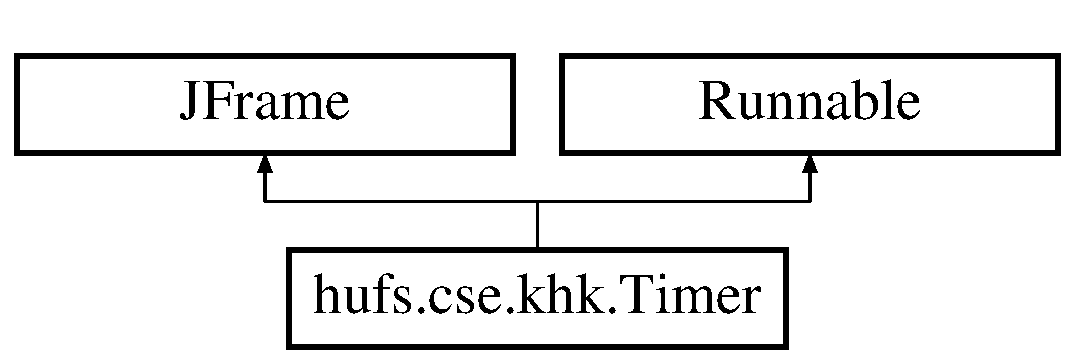
\includegraphics[height=2.000000cm]{classhufs_1_1cse_1_1khk_1_1_timer}
\end{center}
\end{figure}
\subsection*{Public 멤버 함수}
\begin{DoxyCompactItemize}
\item 
\hyperlink{classhufs_1_1cse_1_1khk_1_1_timer_a25d73bcedd05f48488a8207778c0473f}{Timer} (\hyperlink{classhufs_1_1cse_1_1khk_1_1_minesweeper_u_i}{Minesweeper\+UI} minesweeperui)
\begin{DoxyCompactList}\small\item\em 생성자 \end{DoxyCompactList}\item 
void \hyperlink{classhufs_1_1cse_1_1khk_1_1_timer_a9d5cbcd099fbf45ee12465c31aa8a900}{run} ()
\begin{DoxyCompactList}\small\item\em run timer \end{DoxyCompactList}\item 
void \hyperlink{classhufs_1_1cse_1_1khk_1_1_timer_aa688344595bf7a0776ea1907715ca592}{Start} ()
\begin{DoxyCompactList}\small\item\em Start timer. \end{DoxyCompactList}\item 
long \hyperlink{classhufs_1_1cse_1_1khk_1_1_timer_a5ab9e7bd1e1b1f74604887cd99b27972}{stop} ()
\begin{DoxyCompactList}\small\item\em stop timer \end{DoxyCompactList}\end{DoxyCompactItemize}
\subsection*{Private 멤버 함수}
\begin{DoxyCompactItemize}
\item 
void \hyperlink{classhufs_1_1cse_1_1khk_1_1_timer_a8f8ef7cc5071b83bf067ec1e869a3784}{display\+Elapsed\+Time} (long user\+\_\+time)
\begin{DoxyCompactList}\small\item\em display update \end{DoxyCompactList}\end{DoxyCompactItemize}


\subsection{상세한 설명}
\hyperlink{classhufs_1_1cse_1_1khk_1_1_timer}{Timer} Class. 

\begin{DoxyAuthor}{작성자}
gudrbscse
\end{DoxyAuthor}
User 의 Game 진행 시간을 저장하는 클래스이다. 

Timer.\+java 파일의 13 번째 라인에서 정의되었습니다.



\subsection{생성자 \& 소멸자 문서화}
\index{hufs\+::cse\+::khk\+::\+Timer@{hufs\+::cse\+::khk\+::\+Timer}!Timer@{Timer}}
\index{Timer@{Timer}!hufs\+::cse\+::khk\+::\+Timer@{hufs\+::cse\+::khk\+::\+Timer}}
\subsubsection[{\texorpdfstring{Timer(\+Minesweeper\+U\+I minesweeperui)}{Timer(MinesweeperUI minesweeperui)}}]{\setlength{\rightskip}{0pt plus 5cm}hufs.\+cse.\+khk.\+Timer.\+Timer (
\begin{DoxyParamCaption}
\item[{{\bf Minesweeper\+UI}}]{minesweeperui}
\end{DoxyParamCaption}
)}\hypertarget{classhufs_1_1cse_1_1khk_1_1_timer_a25d73bcedd05f48488a8207778c0473f}{}\label{classhufs_1_1cse_1_1khk_1_1_timer_a25d73bcedd05f48488a8207778c0473f}


생성자 


\begin{DoxyParams}{매개변수}
{\em minesweeperui} & \\
\hline
\end{DoxyParams}
생성자를 통해서 ui class 를 받는다. 

Timer.\+java 파일의 26 번째 라인에서 정의되었습니다.


\begin{DoxyCode}
26                                              \{
27         this.minesweeperui = minesweeperui;
28     \}
\end{DoxyCode}


\subsection{멤버 함수 문서화}
\index{hufs\+::cse\+::khk\+::\+Timer@{hufs\+::cse\+::khk\+::\+Timer}!display\+Elapsed\+Time@{display\+Elapsed\+Time}}
\index{display\+Elapsed\+Time@{display\+Elapsed\+Time}!hufs\+::cse\+::khk\+::\+Timer@{hufs\+::cse\+::khk\+::\+Timer}}
\subsubsection[{\texorpdfstring{display\+Elapsed\+Time(long user\+\_\+time)}{displayElapsedTime(long user_time)}}]{\setlength{\rightskip}{0pt plus 5cm}void hufs.\+cse.\+khk.\+Timer.\+display\+Elapsed\+Time (
\begin{DoxyParamCaption}
\item[{long}]{user\+\_\+time}
\end{DoxyParamCaption}
)\hspace{0.3cm}{\ttfamily [private]}}\hypertarget{classhufs_1_1cse_1_1khk_1_1_timer_a8f8ef7cc5071b83bf067ec1e869a3784}{}\label{classhufs_1_1cse_1_1khk_1_1_timer_a8f8ef7cc5071b83bf067ec1e869a3784}


display update 

UI 의 time display 를 update 하게 해준다. 

Timer.\+java 파일의 75 번째 라인에서 정의되었습니다.



다음을 참조함 \+:  hufs.\+cse.\+khk.\+Timer.\+run().



다음에 의해서 참조됨 \+:  hufs.\+cse.\+khk.\+Timer.\+stop().


\begin{DoxyCode}
75                                                     \{
76         \textcolor{keywordflow}{if} (user\_time >= 0 && user\_time < 9) \{
77             minesweeperui.time\_count.setText(\textcolor{stringliteral}{"00"} + user\_time);
78         \} \textcolor{keywordflow}{else} \textcolor{keywordflow}{if} (user\_time > 9 && user\_time < 99) \{
79             minesweeperui.time\_count.setText(\textcolor{stringliteral}{"0"} + user\_time);
80         \} \textcolor{keywordflow}{else} \textcolor{keywordflow}{if} (user\_time > 99 && user\_time < 999) \{
81             minesweeperui.time\_count.setText(\textcolor{stringliteral}{""} + user\_time);
82         \}
83     \}
\end{DoxyCode}
\index{hufs\+::cse\+::khk\+::\+Timer@{hufs\+::cse\+::khk\+::\+Timer}!run@{run}}
\index{run@{run}!hufs\+::cse\+::khk\+::\+Timer@{hufs\+::cse\+::khk\+::\+Timer}}
\subsubsection[{\texorpdfstring{run()}{run()}}]{\setlength{\rightskip}{0pt plus 5cm}void hufs.\+cse.\+khk.\+Timer.\+run (
\begin{DoxyParamCaption}
{}
\end{DoxyParamCaption}
)}\hypertarget{classhufs_1_1cse_1_1khk_1_1_timer_a9d5cbcd099fbf45ee12465c31aa8a900}{}\label{classhufs_1_1cse_1_1khk_1_1_timer_a9d5cbcd099fbf45ee12465c31aa8a900}


run timer 

1초 단위로 시간이 동작하게 하는 함수이다. 

Timer.\+java 파일의 33 번째 라인에서 정의되었습니다.



다음에 의해서 참조됨 \+:  hufs.\+cse.\+khk.\+Timer.\+display\+Elapsed\+Time().


\begin{DoxyCode}
33                       \{
34         \textcolor{keywordflow}{try} \{
35             \textcolor{keywordflow}{while} (isRunning) \{
36                 SwingUtilities.invokeAndWait(displayUpdater);
37                 Thread.sleep(1000);
38             \}
39         \} \textcolor{keywordflow}{catch} (java.lang.reflect.InvocationTargetException ite) \{
40             ite.printStackTrace(System.err);
41         \} \textcolor{keywordflow}{catch} (InterruptedException ie) \{
42         \}
43     \}
\end{DoxyCode}
\index{hufs\+::cse\+::khk\+::\+Timer@{hufs\+::cse\+::khk\+::\+Timer}!Start@{Start}}
\index{Start@{Start}!hufs\+::cse\+::khk\+::\+Timer@{hufs\+::cse\+::khk\+::\+Timer}}
\subsubsection[{\texorpdfstring{Start()}{Start()}}]{\setlength{\rightskip}{0pt plus 5cm}void hufs.\+cse.\+khk.\+Timer.\+Start (
\begin{DoxyParamCaption}
{}
\end{DoxyParamCaption}
)}\hypertarget{classhufs_1_1cse_1_1khk_1_1_timer_aa688344595bf7a0776ea1907715ca592}{}\label{classhufs_1_1cse_1_1khk_1_1_timer_aa688344595bf7a0776ea1907715ca592}


Start timer. 

마우스가 지뢰를 찾기 시작하면 timer 를 시작해주는 함수이다. 

Timer.\+java 파일의 49 번째 라인에서 정의되었습니다.



다음에 의해서 참조됨 \+:  hufs.\+cse.\+khk.\+Minesweeper\+U\+I.\+action\+Performed().


\begin{DoxyCode}
49                         \{
50         startTime = System.currentTimeMillis();
51         isRunning = \textcolor{keyword}{true};
52         updater = \textcolor{keyword}{new} Thread(\textcolor{keyword}{this});
53         updater.start();
54     \}
\end{DoxyCode}
\index{hufs\+::cse\+::khk\+::\+Timer@{hufs\+::cse\+::khk\+::\+Timer}!stop@{stop}}
\index{stop@{stop}!hufs\+::cse\+::khk\+::\+Timer@{hufs\+::cse\+::khk\+::\+Timer}}
\subsubsection[{\texorpdfstring{stop()}{stop()}}]{\setlength{\rightskip}{0pt plus 5cm}long hufs.\+cse.\+khk.\+Timer.\+stop (
\begin{DoxyParamCaption}
{}
\end{DoxyParamCaption}
)}\hypertarget{classhufs_1_1cse_1_1khk_1_1_timer_a5ab9e7bd1e1b1f74604887cd99b27972}{}\label{classhufs_1_1cse_1_1khk_1_1_timer_a5ab9e7bd1e1b1f74604887cd99b27972}


stop timer 

game 이 끝나면 user 의 time 을 반환해 준다. \begin{DoxyReturn}{반환값}
user\+\_\+time 
\end{DoxyReturn}


Timer.\+java 파일의 60 번째 라인에서 정의되었습니다.



다음을 참조함 \+:  hufs.\+cse.\+khk.\+Timer.\+display\+Elapsed\+Time().



다음에 의해서 참조됨 \+:  hufs.\+cse.\+khk.\+Minesweeper\+U\+I.\+Minesweeper\+U\+I(), hufs.\+cse.\+khk.\+Minesweeper\+U\+I.\+Search\+Mine(), hufs.\+cse.\+khk.\+Minesweeper\+U\+I.\+setmenu(), hufs.\+cse.\+khk.\+Minesweeper\+U\+I.\+win\+\_\+check().


\begin{DoxyCode}
60                        \{
61         \textcolor{keywordtype}{long} user\_time = timer;
62         isRunning = \textcolor{keyword}{false};
63         \textcolor{keywordflow}{try} \{
64             updater.join();
65         \} \textcolor{keywordflow}{catch} (InterruptedException ie) \{
66         \}
67         \hyperlink{classhufs_1_1cse_1_1khk_1_1_timer_a8f8ef7cc5071b83bf067ec1e869a3784}{displayElapsedTime}(user\_time);
68         timer = 0;
69         \textcolor{keywordflow}{return} user\_time;
70     \}
\end{DoxyCode}


이 클래스에 대한 문서화 페이지는 다음의 파일로부터 생성되었습니다.\+:\begin{DoxyCompactItemize}
\item 
C\+:/pub/\+Workspace\+\_\+\+S\+E/\+Report3\+\_\+test3/src/hufs/cse/khk/\hyperlink{_timer_8java}{Timer.\+java}\end{DoxyCompactItemize}

\chapter{파일 문서화}
\hypertarget{main_8java}{}\section{C\+:/pub/\+Workspace\+\_\+\+S\+E/\+Report3\+\_\+test3/src/hufs/cse/khk/main.java 파일 참조}
\label{main_8java}\index{C\+:/pub/\+Workspace\+\_\+\+S\+E/\+Report3\+\_\+test3/src/hufs/cse/khk/main.\+java@{C\+:/pub/\+Workspace\+\_\+\+S\+E/\+Report3\+\_\+test3/src/hufs/cse/khk/main.\+java}}
\subsection*{클래스}
\begin{DoxyCompactItemize}
\item 
class \hyperlink{classhufs_1_1cse_1_1khk_1_1main}{hufs.\+cse.\+khk.\+main}
\begin{DoxyCompactList}\small\item\em Run Class. \end{DoxyCompactList}\end{DoxyCompactItemize}
\subsection*{패키지}
\begin{DoxyCompactItemize}
\item 
package \hyperlink{namespacehufs_1_1cse_1_1khk}{hufs.\+cse.\+khk}
\end{DoxyCompactItemize}

\hypertarget{_minesweeper_8java}{}\section{C\+:/pub/\+Workspace\+\_\+\+S\+E/\+Report3\+\_\+test3/src/hufs/cse/khk/\+Minesweeper.java 파일 참조}
\label{_minesweeper_8java}\index{C\+:/pub/\+Workspace\+\_\+\+S\+E/\+Report3\+\_\+test3/src/hufs/cse/khk/\+Minesweeper.\+java@{C\+:/pub/\+Workspace\+\_\+\+S\+E/\+Report3\+\_\+test3/src/hufs/cse/khk/\+Minesweeper.\+java}}
\subsection*{클래스}
\begin{DoxyCompactItemize}
\item 
class \hyperlink{classhufs_1_1cse_1_1khk_1_1_minesweeper}{hufs.\+cse.\+khk.\+Minesweeper}
\begin{DoxyCompactList}\small\item\em \hyperlink{classhufs_1_1cse_1_1khk_1_1_minesweeper}{Minesweeper} \+: \hyperlink{classhufs_1_1cse_1_1khk_1_1_minesweeper}{Minesweeper} data class. \end{DoxyCompactList}\end{DoxyCompactItemize}
\subsection*{패키지}
\begin{DoxyCompactItemize}
\item 
package \hyperlink{namespacehufs_1_1cse_1_1khk}{hufs.\+cse.\+khk}
\end{DoxyCompactItemize}

\hypertarget{_minesweeper_u_i_8java}{}\section{C\+:/pub/\+Workspace\+\_\+\+S\+E/\+Report3\+\_\+test3/src/hufs/cse/khk/\+Minesweeper\+UI.java 파일 참조}
\label{_minesweeper_u_i_8java}\index{C\+:/pub/\+Workspace\+\_\+\+S\+E/\+Report3\+\_\+test3/src/hufs/cse/khk/\+Minesweeper\+U\+I.\+java@{C\+:/pub/\+Workspace\+\_\+\+S\+E/\+Report3\+\_\+test3/src/hufs/cse/khk/\+Minesweeper\+U\+I.\+java}}
\subsection*{클래스}
\begin{DoxyCompactItemize}
\item 
class \hyperlink{classhufs_1_1cse_1_1khk_1_1_minesweeper_u_i}{hufs.\+cse.\+khk.\+Minesweeper\+UI}
\begin{DoxyCompactList}\small\item\em \hyperlink{classhufs_1_1cse_1_1khk_1_1_minesweeper}{Minesweeper} UI. \end{DoxyCompactList}\item 
class {\bfseries hufs.\+cse.\+khk.\+Minesweeper\+U\+I.\+Mouse\+Handler}
\begin{DoxyCompactList}\small\item\em Mouse Handler. \end{DoxyCompactList}\item 
class {\bfseries hufs.\+cse.\+khk.\+Minesweeper\+U\+I.\+Customization}
\begin{DoxyCompactList}\small\item\em Customize Mode. \end{DoxyCompactList}\end{DoxyCompactItemize}
\subsection*{패키지}
\begin{DoxyCompactItemize}
\item 
package \hyperlink{namespacehufs_1_1cse_1_1khk}{hufs.\+cse.\+khk}
\end{DoxyCompactItemize}

\hypertarget{_rank_8java}{}\section{C\+:/pub/\+Workspace\+\_\+\+S\+E/\+Report3\+\_\+test3/src/hufs/cse/khk/\+Rank.java 파일 참조}
\label{_rank_8java}\index{C\+:/pub/\+Workspace\+\_\+\+S\+E/\+Report3\+\_\+test3/src/hufs/cse/khk/\+Rank.\+java@{C\+:/pub/\+Workspace\+\_\+\+S\+E/\+Report3\+\_\+test3/src/hufs/cse/khk/\+Rank.\+java}}
\subsection*{클래스}
\begin{DoxyCompactItemize}
\item 
class \hyperlink{classhufs_1_1cse_1_1khk_1_1_rank}{hufs.\+cse.\+khk.\+Rank}
\begin{DoxyCompactList}\small\item\em \hyperlink{classhufs_1_1cse_1_1khk_1_1_rank}{Rank} \+: User Ranking Class. \end{DoxyCompactList}\end{DoxyCompactItemize}
\subsection*{패키지}
\begin{DoxyCompactItemize}
\item 
package \hyperlink{namespacehufs_1_1cse_1_1khk}{hufs.\+cse.\+khk}
\end{DoxyCompactItemize}

\hypertarget{_timer_8java}{}\section{C\+:/pub/\+Workspace\+\_\+\+S\+E/\+Report3\+\_\+test3/src/hufs/cse/khk/\+Timer.java 파일 참조}
\label{_timer_8java}\index{C\+:/pub/\+Workspace\+\_\+\+S\+E/\+Report3\+\_\+test3/src/hufs/cse/khk/\+Timer.\+java@{C\+:/pub/\+Workspace\+\_\+\+S\+E/\+Report3\+\_\+test3/src/hufs/cse/khk/\+Timer.\+java}}
\subsection*{클래스}
\begin{DoxyCompactItemize}
\item 
class \hyperlink{classhufs_1_1cse_1_1khk_1_1_timer}{hufs.\+cse.\+khk.\+Timer}
\begin{DoxyCompactList}\small\item\em \hyperlink{classhufs_1_1cse_1_1khk_1_1_timer}{Timer} Class. \end{DoxyCompactList}\end{DoxyCompactItemize}
\subsection*{패키지}
\begin{DoxyCompactItemize}
\item 
package \hyperlink{namespacehufs_1_1cse_1_1khk}{hufs.\+cse.\+khk}
\end{DoxyCompactItemize}

%--- End generated contents ---

% Index
\backmatter
\newpage
\phantomsection
\clearemptydoublepage
\addcontentsline{toc}{chapter}{색인}
\printindex

\end{document}
